%%%%%%%%%%%%%%%%%%%%%%%%%%%%%%%%%%%%%%%%%%%%%%%%%%%%%%%%%%%%%%%%%%%%%%%%%
%%   CHAPTER: UNIVERSAL CONSTRUCTION
%%%%%%%%%%%%%%%%%%%%%%%%%%%%%%%%%%%%%%%%%%%%%%%%%%%%%%%%%%%%%%%%%%%%%%%%%

\renewcommand{\chapterfolder}{universal_construction/}
\chapterimage{cover/universal_construction}
\chapter{Universal Construction}\label{chp:universal_construction}


\vspace*{-0.4in}
\epigraph{The truth is you don't know what is going to happen tomorrow. Life is a crazy ride, and nothing is guaranteed.}{Eminem}
\vspace*{0.4in}


\noindent In the previous chapter, we learned that we can often stabilize unstable reactions (like the $31c/240$~reaction of Figure~\ref{fig:31c_240_reaction}, or the $17c/45$~reaction of Figure~\ref{fig:17c45_reaction}) by using them to create gliders, and then using those gliders to synthesize stabilizing components. In this chapter, we take this idea one step further and show that similar behavior can be achieved without the need for the initial unstable reaction---we can use gliders to create or move some component in the Life plane, while simultaneously moving or recreating those gliders so that they can be re-used.

We refer to these techniques as \emph{universal construction},\index{universal construction} and a pattern that implements them as a \emph{universal constructor},\index{universal constructor} with ``universal'' referring to the fact that they can build any Life pattern that is synthesizable via gliders.\footnote{Some patterns, like Gardens of Eden and the grandparentless pattern from Figure~\ref{fig:grandparentless}, cannot be synthesized by gliders.} Although most universal constructors only fire slow glider salvos, we know from Theorem~\ref{thm:p2_slow_salvo} that this is enough to implement arbitrary glider syntheses. Most useful universal constructors are built out of simple stable components like blocks, beehives, and eater~1s, so that it is relatively straightforward to synthesize them via gliders, and thus they can even be used to build copies of themselves.


%%%%%%%%%%%%%%%%%%%%%%%%%%%%%%%%
\section{Gemini}\label{sec:gemini}\index{gemini}
%%%%%%%%%%%%%%%%%%%%%%%%%%%%%%%%

% As our first illustration of the utility of universal computation...

% TODO: Describe the general shape of Gemini a bit better first? Spaceship that builds itself in front of itself.

We have seen the basic idea behind universal construction several times now, starting back in Section~\ref{sec:slide_guns}. By using a sliding block (or other small still life) as an elbow, we can fire gliders at any location in the Life plane, thus allowing a sequence of gliders to encode the construction or destruction of essentially any pattern (via the slow salvo techniques of Section~\ref{sec:slow_salvo}, for example).


%%%%%%%%%%%%%%%%%%%%%%%%%%%%%%%%
\subsection{Elbow Operations}\label{sec:gemini_elbow}
%%%%%%%%%%%%%%%%%%%%%%%%%%%%%%%%

We already saw gliders salvos that push or pull a sliding block back in Figure~\ref{fig:synchronized_block_movers}, as well as salvos that can be used to fire perpendicular gliders of either color in Figure~\ref{fig:synchronized_block_reflectors}. We summarize those reactions that we will make use of in Figure~\ref{fig:gemini_glider_operations},\footnote{The names ``\texttt{FIRE WHITE}'' and ``\texttt{FIRE BLACK}'' used for two of these reactions just refer to the fact that they fire perpendicular gliders of opposite colors (the absolute color names do not matter).} noting that just these four operations are enough for us to be able to implement any unidirectional slow salvo of our choosing.% Footnote about only needing 3?

\begin{figure}[!htb]
	\centering
	\begin{tabular}{@{}cccc@{}}
		\begin{subfigure}{0.23\textwidth}
			\centering
			\patternimglink{0.12}{gemini_pull}
			\caption{\texttt{PULL}}
			\label{fig:gemini_pull}
		\end{subfigure} & \begin{subfigure}{0.23\textwidth}
			\centering
			\patternimglink{0.12}{gemini_push}
			\caption{\texttt{PUSH}}
			\label{fig:gemini_push}
		\end{subfigure} & \begin{subfigure}{0.23\textwidth}
			\centering
			\patternimglink{0.12}{gemini_fire_white}
			\caption{\texttt{FIRE WHITE}}
			\label{fig:gemini_fire_white}
		\end{subfigure} & \begin{subfigure}{0.23\textwidth}
			\centering
			\patternimglink{0.12}{gemini_fire_black}
			\caption{\texttt{FIRE BLACK}}
			\label{fig:gemini_fire_black}
		\end{subfigure}
	\end{tabular}
	\caption{A collection of reactions that can be used to fire perpendicular gliders (to the southwest) along any lane of our choosing. All four reactions use the same initial pair of gliders (highlighted in \bgbox{orangeback2}{orange}).}\label{fig:gemini_glider_operations}
\end{figure}

By using some Herschel circuitry to create these glider configurations, we can straightforwardly construct the component displayed in Figure~\ref{fig:construction_arm} that takes an input glider on one of four different lanes and performs the corresponding operation on  the sliding block. This particular component uses some slightly old conduits like Silver reflectors (refer back to Figure~\ref{fig:silver_reflector}) rather than more recent conduits for two reasons: (1) it will be useful for us to have this component built entirely out of pieces like blocks and eater~1s (and unlike Snarks) that are ``simple'' to synthesize, and (2) the Gemini spaceship that we will construct out of this component was built before many of the more efficient conduits that we have explored.\footnote{For example, the Gemini spaceship that we will soon construct was built in 2010, whereas the Snark was found in 2013 and the syringe was found in 2015.}

\begin{figure}[!htb]
	\centering
	\embedlink{construction_arm}{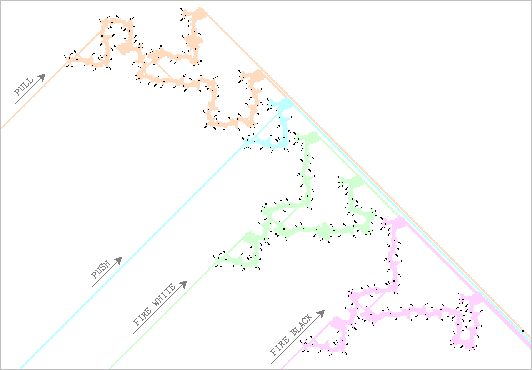
\includegraphics[width=\textwidth]{universal_construction/construction_arm.pdf}}
	\caption{An elbow-operation circuit, which takes a glider on one of four input glider lanes and as a result either pulls or pushes the sliding block (elbow), or uses it to fire a perpendicular glider of either color to the southwest. Note that all four actions require the \texttt{PULL} circuit to be activated, as it produces the frontmost pair of gliders in all four operations (see Exercise~\ref{exer:construction_arm_lanes_timed}). Constructed by Paul Chapman in 2004.}\label{fig:construction_arm}
\end{figure}

By aiming the output gliders of two of these elbow-operation circuits at each other, we can encode the construction of any glider-synthesizable pattern in the input streams (with the advantage that the input lanes are fixed, whereas the output lanes are not).\footnote{This is similar to how we encoded the synthesis of a $2$-engine Cordership in some glider sequences back in Figure~\ref{fig:armless_cordership_gun}.} For example, the pattern displayed in Figure~??...

% FIGURE


%%%%%%%%%%%%%%%%%%%%%%%%%%%%%%%%
\subsection{The Spaceship Itself}\label{sec:gemini_itself}
%%%%%%%%%%%%%%%%%%%%%%%%%%%%%%%%

Importantly, because these circuits are made up of such simple components (mostly blocks and eater~1s, with the most difficult piece to synthesize being a tub), they can even be used to synthesize copies of \emph{themselves}. Indeed, this is the key idea behind the Gemini spaceship: use an extremely long chain of gliders to have two of these circuits build copies of themselves somewhere else in the plane. To turn this idea into a \emph{spaceship} though (rather than just something that repeatedly builds copies of itself), we need to make two additions:\smallskip

\begin{itemize}
	\item[1)] We need to destroy the original pair of elbow-operation circuits after they have constructed the new ones. To do this, we simply use a third elbow-operation circuit, which is constructed alongside the original pair. After all three circuits are constructed, the first two start construction again while the third one starts destroying the old circuits. Since objects like blocks and eater~1s can easily be destroyed by a single glider each, it is straightforward to find a glider recipe that destroys the elbow-operation circuits.\smallskip
	
	\item[2)] We need to be able to re-use the glider recipes that store the construction and destruction recipes. Since we cannot use a static loop (we need the glider recipes to move along with the elbow-operation circuits), we instead have the glider recipes bounce back and forth between \emph{two} copies of the entire three-elbow-operation circuit that we have described.\footnote{In fact, the two ends of the spaceship that we construct will be exactly identical. This is the reason for its name ``Gemini''---it is Latin for ``twins''.}\smallskip
\end{itemize}

After we put all of these ideas together, we get the Gemini spaceship that is displayed in Figure~\ref{fig:gemini}.\footnote{Constructed by Andrew Wade in May 2010.} It builds a copy of itself displaced by 5,120 cells in one direction and 1,024 cells in the other direction every 33,699,586 generations, making it the first spaceship that we have seen that does not travel orthogonally or diagonally at a slope of~$1$ (its slope is $5120/1024 = 5$).

\begin{figure}[!htbp]
	\centering
	\embedlink{gemini}{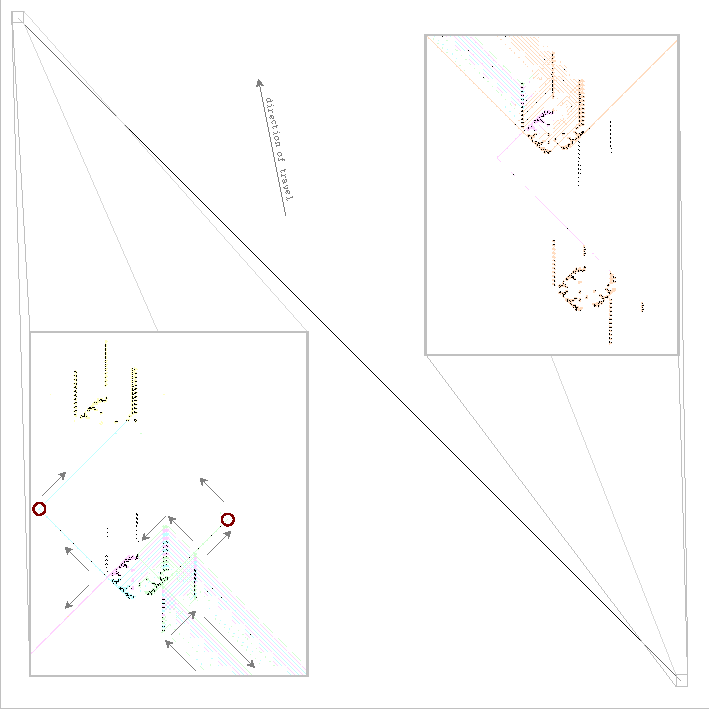
\includegraphics[width=\textwidth]{universal_construction/gemini.pdf}}
	\caption{The self-constructing \emph{Gemini} spaceship, which simply looks like a long, thin diagonal line when zoomed out far enough to see in its entirety. The bulk of the spaceship of made up of 24 parallel glider lanes (12 travelling in each direction), which carry a recipe for building the ship. The ends of the spaceship, which are zoomed in on here, are identical arrangements of stable glider reflectors, glider duplicators, and three elbow-operation circuits whose sliding blocks are circled in \bgbox{redback}{red}. The elbow-operation circuits highlighted in \bgbox{aquaback}{aqua} and \bgbox{greenpastel}{green} build the next copy of the spaceship (highlighted in \bgbox{yellowback2}{yellow}), while the elbow-operation circuit higlighted in \bgbox{magentaback}{magenta} destroys the previous copy of the spaceship (highlighted in \bgbox{orangeback2}{orange}).}\label{fig:gemini}
\end{figure}


%%%%%%%%%%%%%%%%%%%%%%%%%%%%%%%%
\subsection{Geminoids}\label{sec:geminoids}
%%%%%%%%%%%%%%%%%%%%%%%%%%%%%%%%

Stuff.
% Describe how fast we can make it go, what the limiting factor is. Say not worth showing variations in bookks since they look essentially identical.


%%%%%%%%%%%%%%%%%%%%%%%%%%%%%%%%
\section{Demonoids}\label{sec:demonoid}
%%%%%%%%%%%%%%%%%%%%%%%%%%%%%%%%

Stuff.

\begin{figure}[!htb]
	\centering
	\patternimglink{0.1}{demonoid}
	\caption{A demonoid. Just testing some stuff for now.}\label{fig:demonoid}
\end{figure}



%%%%%%%%%%%%%%%%%%%%%%%%%%%%%%%%
\section*{Notes and Historical Remarks}
%%%%%%%%%%%%%%%%%%%%%%%%%%%%%%%%

Stuff.
% TAlk about Gemini took 5 months to complete. Maybe earlier instead. Made with a custom computer script to make the glider recipe


% BUILD A GEMINI WITH DIFFERENT PERIOD/SLOPE/WHATEVER
%%%%%%%%%%%%%%%%%%%%%%%%%%%%%%%%%
\section*{Exercises \hfill \normalfont\textsf{\small solutions to starred exercises on \hyperlink{solutions_universal_construction}{page \pageref{solutions_universal_construction}}}}
\label{sec:universal_construction_exercises}
\addcontentsline{toc}{section}{Exercises}
\vspace*{-0.4cm}\hrulefill\vspace*{-0.3cm}\footnotesize\begin{multicols}{2}\vspace*{-0.4cm}\raggedcolumns\interlinepenalty=10000
\setlength{\parskip}{0pt}
%%%%%%%%%%%%%%%%%%%%%%%%%%%%%%%%%


\begin{problem}\label{exer:construction_arm_lanes_timed}
	The elbow-operation circuit of Figure~\ref{fig:construction_arm} requires two synchronized input gliders to trigger each of the \texttt{PUSH}, \texttt{FIRE WHITE}, and \texttt{FIRE BLACK} operations---one to create the frontmost pair of gliders via the \texttt{PULL} circuit, and one to create the additional glider(s).
	
	Add additional Herschel conduits to that circuit so that each of the four operations can be triggered by just a single input glider.
\end{problem}


\mfilbreak


\begin{problemstar}\label{exer:gemini_unhighlighted_reflectors}
	The two zoom boxes in Figure~\ref{fig:gemini} each have two rows of unhighlighted reflectors that never reflect a single glider. What is their purpose?
\end{problemstar}


%% EXERCISE END COMMANDS
\end{multicols}
\normalsize\vspace*{0.01cm}
%% DONE EXERCISE END COMMANDS